\documentclass[titlepage=firstiscover, captions=tableheading, bibliography=totoc]{scrartcl}
\usepackage[autostyle=true,german=quotes]{csquotes}
\usepackage{scrhack}
\usepackage{caption}
\usepackage[aux]{rerunfilecheck}
\usepackage{subcaption}        
\usepackage{fontspec}
\usepackage[dvips]{graphicx}
\usepackage{floatflt,epsfig} 
    
\usepackage{polyglossia}
\setmainlanguage{german}

\usepackage[unicode]{hyperref}
\usepackage{bookmark}
\title{V27\\ Der Helium-Neon-Laser}
\author{
Miriam Simm\\
\texorpdfstring{\href{mailto:miriam.simm@tu-dortmund.de}{miriam.simm@tu-dortmund.de}\and}{,}
Katrin Bolsmann\\
\texorpdfstring{\href{mailto:katrin.bolsmann@tu-dortmund.de}{katrin.bolsmann@tu-dortmund.de}}{}
}
\date{Durchführung: 15.06.2020 \\ Abgabe: -.06.2020}
\usepackage{amsmath} 
\usepackage{amssymb} 
\usepackage{mathtools}
\usepackage[
    math-style=ISO,
    bold-style=ISO,
    sans-style=italic,
    nabla=upright,
    partial=upright,
]{unicode-math}
    
\setmathfont{Latin Modern Math}

\usepackage[
  locale=DE,
  separate-uncertainty=true, 
  per-mode=symbol-or-fraction,
]{siunitx}

\usepackage{multicol}
\setlength{\columnsep}{1pt} %space between columns 

\usepackage{booktabs}
\usepackage[x11names, table]{xcolor}
\usepackage{graphicx}
\usepackage{grffile}
\usepackage{xfrac}
\usepackage{xcolor}

\usepackage{float}
\floatplacement{figure}{h}
\floatplacement{table}{h}
\usepackage[
  section,
  below,
]{placeins}

\usepackage{expl3}
\usepackage{xparse}
\ExplSyntaxOn
\NewDocumentCommand \E {} {\symup{e}}
\ExplSyntaxOff

% Literaturverzeichnis
\usepackage[
  backend=biber,
]{biblatex}
% Quellendatenbank
\addbibresource{literatur.bib}

\usepackage[
  version=4,
  math-greek=default,
  text-greek=default,
]{mhchem}
 

\raggedcolumns

\begin{document}

\maketitle
\thispagestyle{empty}
\tableofcontents
\newpage

\section{Zielsetzung}
Ziel dieses Versuches ist die Untersuchung der Spektren von unbekannten Strahlern bezüglich der Energie und Aktivität.
Hierzu werden zuerst die Detektoreigenschaften anhand bekannter Strahler bestimmt. 

\section{Theorie}
\subsection{Wechselwirkung von Gamma-Strahlung mit Materie}
Durch Wechselwirkung mit Materie wird die Ausbreitungsrichtung der Gamma-Quanten geändert oder diese werden annihiliert, sodass die Intensität gemäß des Lambert-Beerschen-Gesetzes
\begin{equation}
I(x) = I_0 \exp(-\mu x)
\end{equation}
abnimmt,
wobei $I_0$ der ursprünglichen Intensität und $x$ der zurückgelegten Strecke im Medium entspricht.
Die mittlere Reichweite der Gamma-Strahlung in diesem Medium entspricht dem Kehrwert des Extinktionskoeffizienten, welcher sich mit der Ordnungszahl $Z$, der Teilchenzahldichte $n$ und dem Wirkungsquerschnitt $\sigma$ gemäß der Formel
\begin{equation}\label{eq:mu}
\mu = Zn\sigma
\end{equation}
beschreiben lässt.

\FloatBarrier
\begin{figure}[h]
\begin{minipage}[t]{0.48\textwidth}
\vspace{0pt}
Der Wirkungsquerschnitt setzt sich wiederum aus verschiedenen Wechselwirkungen zusammen, welche je nach Energie verschieden starke Beiträge liefern.
So dominiert bei geringeren Energien der Photoeffekt, während bei hohen Energien die Paarbildung den größten Beitrag des Wirkungsquerschnittes liefert.
Der Compton-Effekt ist bei fast allen Energien präsent, liefert jedoch nur für Energien zwischen $100\, \si{\keV}$ und $10\,\si{\MeV}$ einen relevanten Beitrag.
In Abbildung \ref{fig:tfig1} ist der Verlauf des Extinktionskoeffizienten $\mu$ dargestellt.
Da es sich bei den in Abbildung \ref{fig:tfig1} beschriebenen Prozessen um die drei wichtigsten Prozesse bezogen auf Absorption von Gamma-Strahlung in Materie handelt, sollen diese im Folgenden genauer erläutert werden.
\end{minipage}
\hfill
\begin{minipage}[t]{0.50\textwidth}
\vspace{-10pt}
\centering
\includegraphics[width=\textwidth]{Absorption.png}
\caption{Der Extinktionskoeffizient in Abhängigkeit der Energie für verschiedene Wechselwirkungsprozesse: Photoeffekt, Comptoneffekt und Paarbildung \cite{quelle02}.}
\label{fig:tfig1}
\end{minipage}
\end{figure}
\FloatBarrier

\subsubsection*{Der Photoeffekt}
Der Photoeffekt beschreibt die Wechselwirkung eines Gamma-Quants mit einem Hüllenelektron, welches vorzugsweise aus der K-Schale stammt.
Bei diesem Prozess absorbiert das Elektron die gesamte Energie des Photons, sodass dieses annihiliert wird.
\FloatBarrier
\begin{figure}[h]
\begin{minipage}[t]{0.4\textwidth}
\vspace{0pt}
\centering
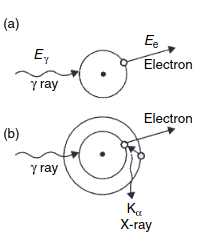
\includegraphics[width=1.1\textwidth]{Photoeffekt.png}
\caption{Der Photoeffekt ohne (a) und mit (b) Emission eines Photons \cite{quelle02}.}
\label{fig:tfig2}
\end{minipage}
\hfill
\begin{minipage}[t]{0.58\textwidth}
\vspace{0pt}
Unter der Vorraussetzung, dass die Energie des Photons größer ist als die Bindungsenergie des Elektrons, wird dieses aus der Elektronenhülle gelöst.
Die restliche Energie wird dem Elektron als kinetische Energie übertragen.
Das vom Elektron hinterlassene Loch in der Elektronenschale wird durch eine Kaskade an Elektronenübergängen erneut besetzt.
Bei diesem Prozess besetzen nacheinander Elektron aus höherenergetischen Schalen das Loch der nächst-tieferen Schale und hinterlassen somit wiederum ein Loch.
Jeder dieser Übergangsprozesse emittiert ein Photon, welches genau der Energiedifferenz der beiden Schalen entspricht und somit dem Spektrum der Röntgenstrahlung zugeordnet wird.
Aufgrund der geringen Reichweite der Röntgenstrahlung kann angenommen werden, dass durch den Photoeffekt die gesamte Energie des Photons im Detektor verbleibt und detektiert werden kann.
\end{minipage}
\end{figure}
\FloatBarrier

Unter der Annahme, dass die Photonenenergie im Bereich des Photoeffektes größer als die Bindungsenergie des Elektrons aber klein gegenüber der Elektronenmasse $m_ec^2$ ist, ist eine nichtrelativistische Näherung gerechtfertigt.
Außerdem wird von der Born'schen Näherung ausgegangen, welche eine ebene Welle für das freigesetzte Elektron annimmt.
Somit kann der Wirkungsquerschnitt des Photoeffektes näherungsweise durch die Formel \cite{quelle03}
\begin{equation}
\sigma_{\text{Ph}}=\sqrt{32}\alpha^4 \varepsilon^\frac{7}{2}Z^5\sigma_{Th}\, , \qquad \varepsilon = \frac{E_{\gamma}}{m_e c^2}
\end{equation}
beschrieben werden.
Hierbei ist $\alpha = \frac{1}{137}$ die Feinstrukturkonstante und $\sigma_{\text{Th}}=\frac{8}{3}\pi r_e^2$ der Thomson-Wirkungsquerschnitt mit dem klassischen Elektronenradius $r_e$.

\subsubsection*{Der Comptoneffekt}
Als Comptoneffekt wird die Streuung eines Photons an einem freien Elektron oder einem quasifreien Hüllenelektron bezeichnet.
Aus Energie- und Impulserhaltung errechnet sich für die Energie des gestreuten Photons in Abhängigkeit des Streuwinkels der Zusammenhang
\begin{equation}
E'_{\gamma} = \frac{E_{\gamma}}{1 + \varepsilon(1-\cos(\theta))} \, .
\end{equation}
Somit ergibt sich für einen Streuwinkel von $\theta = 180°$ der maximale Energieübertrag von
\begin{equation}
\label{eq:compton}
\increment E_\text{max} = \frac{2\varepsilon}{1 + 2 \varepsilon} E_{\gamma} \, .
\end{equation}
Offensichtlich kann das Photon durch die Compton-Wechselwirkung nicht seine gesamte Energie auf das Elektron übertragen, sodass das es bei diesem Prozess nicht annihiliert wird.
Somit ist das Energiespektrum der gestreuten Elektronen kontinuierlich und wird auch Compton-Kontinuum genannt. 
Bei der Maximalenergie, welche für $\theta = 180°$ übertragen wird, bricht dieses abrupt ab und bildet die Comptonkante.
Der Compton-Effekt ist schematisch in Abbildung \ref{fig:tfig4} dargestellt.

\begin{figure}
\centering
\begin{subfigure}{0.55\textwidth}
\centering
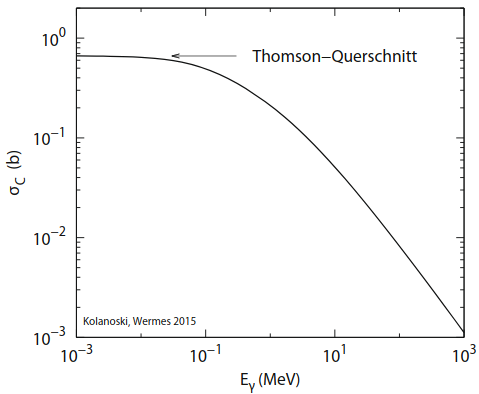
\includegraphics[width=1.03\textwidth]{compton2.png}
\captionsetup{format=hang, labelfont = bf, textfont = small}
\caption{Compton-Wirkungsquerschnitt pro Hüllenelektron gegen die Energie des Photons aufgetragen \cite{quelle03}.}
\label{fig:tfig3}
\end{subfigure}
\begin{subfigure}{0.42\textwidth}
\vspace{35pt}
\centering
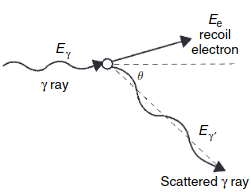
\includegraphics[width=0.9\textwidth]{Compton.png}
\vspace{39pt}
\captionsetup{format=hang, labelfont = bf, textfont = small}
\caption{Schematische Darstellung des Compton-Effekts \cite{quelle02}.}
\label{fig:tfig4}
\end{subfigure}
\caption{Schematische Darstellung der Kinematik des Compton-Effekts, sowie der Energieabhängigkeit des Wirkungsquerschnittes pro Hüllenelektron.}
\vspace{15pt}
\label{fig:tfig34}
\end{figure}
\noindent
Der differentielle Wirkungsquerschnitt wird durch die Klein-Nishina-Formel
\begin{equation}
    \label{eq:diffwirkung}
\frac{d \sigma_C}{dE} = \frac{3}{8}\frac{\sigma_{\text{Thomson}}}{m_e c^2 \varepsilon^2}\left(2+\left(\frac{E}{E_{\gamma}-E}\right)^2
\left(\frac{1}{\varepsilon^2}+\frac{E_{\gamma}-E}{E_{\gamma}}-\frac{2}{\varepsilon}\frac{E_{\gamma}-E}{E_{\gamma}}\right)\right)
\end{equation}
beschrieben. 
Durch Integration ergibt sich für den totalen Wirkungsquerschnitt pro Elektron \cite{quelle03}
\begin{equation}
\sigma_C = 2\pi r_e^2\left[\frac{1+\varepsilon}{\varepsilon^2}\left(\frac{2(1+\varepsilon)}{1+2\varepsilon}-\frac{1}{\varepsilon}\ln(1+2\varepsilon)\right)
+\frac{1}{2\varepsilon}\ln(1+2\varepsilon)-\frac{1+3\varepsilon}{(1+2\varepsilon)^2}\right]\, .
\end{equation}
Somit gilt für den totalen Wirkungsquerschnitts eines Atoms der Kernladungszahl $Z$ der Zusammenhang
\begin{equation}
\sigma_C^{\text{Atom}} = Z \sigma_C \sim \frac{Z}{E_{\gamma}}\, .
\end{equation}
In Abbildung \ref{fig:tfig3} ist der Verlauf des Compton-Wirkungsquerschnittes in Abhängigkeit von der Photonenenergie dargestellt.

\subsubsection*{Die Paarerzeugung}\label{sec:paar}
Ist die Photonenenergie größer als die doppelte Ruhenergie eines Elektrons kommt es zur Erzeugung eines Elektron-Positron-Paares.
Hierbei wird die gesamte Energie des Photons in die Ruheenergie des Elektrons und Positrons, sowie dessen kinetische Energien umgewandelt.
Damit der Impuls erhalten bleibt, bedarf es eines weiteren Stoßpartners, bei dem es sich meistens um einen Atomkern des Absorbermaterials handelt.

Das Positron annihiliert kurz nach seiner Entstehung mit einem im Detektor vorhandenen Elektron, sodass zwei Photonen entstehen.
Die Gesamtenergie des Photons verbleibt nur dann vollständig im Detektor, wenn diese beiden Photonen und das Elektron ebenso dort verbleiben.
Es besteht jedoch eine endliche Wahrscheinlichkeit, dass ein Teil der Energie aus dem Detektor entweicht.
Entweicht eins von den beiden Photonen, wird von einem Single escape gesprochen, das Entweichen beider Photonen wird dementsprechend Double escape genannt.

Der Wirkungsquerschnitt ist davon abhängig, wie stark der Atomkern von den Elektronenhüllen abgeschirmt wird, daher werden zwei Fälle unterschieden:
\begin{align}
\intertext{$\qquad\bullet$ geringe Abschirmung: } \sigma_{\text{Paar}}&=4Z^2 \alpha r_e^2 \left(\frac{7}{9}\ln\left(2\varepsilon\right)-\frac{109}{54}\right)\\
\intertext{$\qquad\bullet$ vollständige Abschirmung: } \sigma_{\text{Paar}}&=4Z^2 \alpha r_e^2 \left(\frac{7}{9}\ln\left(\frac{183}{Z^{1/3}}\right)-\frac{1}{54}\right)
\end{align}
Im Falle vollständiger Abschirmung ist der Wirkungsquerschnitt unabhängig von der Energie des Photons.
Für den Fall geringer Abschirmung ergibt sich ein differentieller Wirkungsquerschnitt von
\begin{equation}
\frac{d\sigma}{d E} = \frac{28\alpha Z² r_e^2}{9E_{\gamma}}\, .
\end{equation}

Abbildung \ref{fig:tfig5} bietet einen Überblick über die drei beschriebenen Wechselwirkungsprozesse der Gamma-Quanten im Detektor.

\FloatBarrier
\begin{figure}
\centering
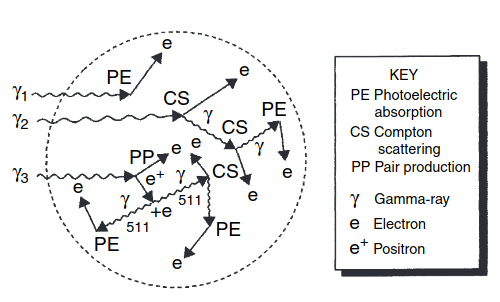
\includegraphics[height=6cm]{alles.png}
\caption{Übersicht der wichtigsten Absorptionsprozesse im Detektor \cite{quelle02}.}
\label{fig:tfig5}
\end{figure}
\FloatBarrier

\subsection{Grundlagen der Halbleiterinstrumente}
Der Germanium-Detektor macht sich einige grundlegende Eigenschaften von dotierten Halbleitern zunutze, welche im Folgenden genauer erläutert werden sollen.

Germanium besitzt 4 Valenzelektronen pro Atom, sodass durch das Einbringen eines Fremdatoms mit 5 Valenzatomen, welches auch Donatoratom genannt wird, sich eins der Elektronen quasifrei bewegen kann und als Ladungsträger dient.
In diesem Fall wird von n-Dotierung gesprochen.
Somit dominieren in einem n-dotierten Halbleiter die Elektronen als Ladungsträger und die Fermienergie liegt nahe am Leitungsband.
Wird stattdessen ein Fremdatom mit 3 Valenzelektronen in das Germanium eingebracht, so entsteht ein Loch, welches als positiver Ladungsträger zur Verfügung steht.
Aufgrund der Eigenschaft des Fremdatoms ein weiteres Elektron binden zu können, werden diese auch Akzeptoren genannt. In diesem Fall liegt ein p-dotierter Halbleiter vor.
In p-dotierten Halbleitern dienen also hauptsächlich Löcher als Ladungsträger und die Fermienergie liegt nahe am Valenzband.

\FloatBarrier
\begin{figure}[h]
\begin{minipage}[t]{0.45\textwidth}
\vspace{10pt}
\centering
\includegraphics[width = 1.05\textwidth]{pnübergang.png}
\caption{Drift und Diffusionstrom an einer pn-Grenzschicht \cite{quelle03}.}
\label{fig:tfig6}
\end{minipage}
\hfill
\begin{minipage}[t]{0.53\textwidth}
\vspace{0pt}
Grenzen p- und n-dotierte Halbleiter direkt aneinander entsteht ein pn-Übergang, wie in Abbildung \ref{fig:tfig6} gezeigt ist.
Aufgrund des Konzentrationsgefälles am pn-Übergang kommt es zu einem Diffusionsstrom, sodass die Donatorelektronen der n-dotierten Seite auf die p-dotierte Seite diffundieren und die Löcher der p-dotierten Seite auf die n-dotierte Seite.
Somit kommt es zu einer Rekombination der Ladungsträger und es bildet sich eine Verarmungszone, in welcher kaum freie Ladungsträger vorhanden sind und die Leitfähigkeit erheblich abnimmt.
Aufgrund der ionisierten Atomrümpfe entsteht eine positive Ladungsdichte an der n-Grenzschicht und eine negative Ladungsdichte an der p-Grenzschicht, sodass sich ein elektrisches Feld ausbildet.
Dieses Feld wirkt wiederum dem Diffusionstrom entgegen, sodass sich ein Gleichgewichtszustand einstellt, in welchem die Verarmungszone eine endliche Breite $d$ besitzt.
\end{minipage}
\end{figure}
\FloatBarrier
Im Allgemeinen ist die Verarmungszone sehr schmal. 
Die Breite kann jedoch durch das Anlegen einer äußeren Spannung vergrößert werden. 
Dies ist essentiell für das hohe Energieauflösevermögen des Germaniumdetektors und wird im folgenden Abschnitt genauer erörtert.

\subsection{Der Halbleiter-Detektor}
In diesem Versuch wird als Detektor ein koaxialer Germanium-Detektor verwendet, welcher in Abbildung \ref{fig:tfig7} abgebildet ist.
Dieser befindet sich unter einer Aluminium-Schutzhaube, sodass die einfallenden Gamma-Quanten mindestens eine Energie von $40 \,\si{keV}$ - $50\,\si{keV}$ besitzen müssen, um diese und die erste Schichte des Detektors überwinden zu können.
Die Oberfläche des Detektors ist mit Lithium-Atomen n-dotiert und besitzt somit eine hohe Leitfähigkeit.
Im Inneren befindet sich eine Bohrung, dessen Oberfläche mit Gold-Atomen p-dotiert ist.
Beide dotierten Schichten dienen zum Anschluss einer äußeren Spannung.
Diese wird so angelegt dass die n-dotierte Schicht für den Anschluss des Pluspols dient.
Durch die angelegte Spannung bildet sich eine ausgedehnte Verarmungszone innerhalb des Detektors, welche den Detektorbereich bildet.

\FloatBarrier
\begin{figure}
\centering
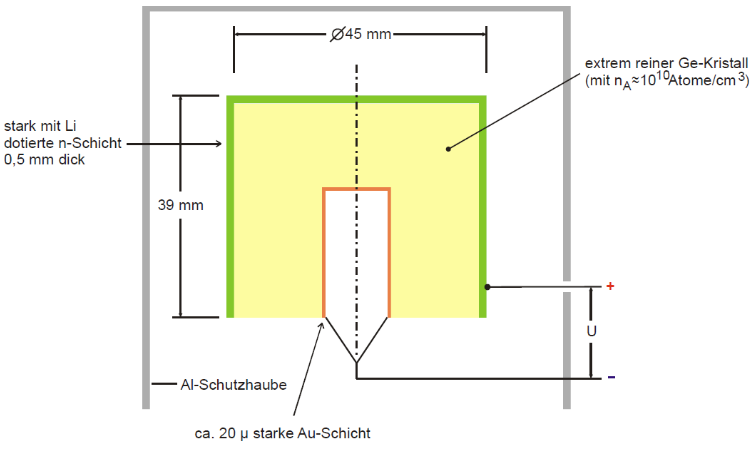
\includegraphics[width = 0.9\textwidth]{Detektor.png}
\caption{Querschnitt des koaxialen Germaniumdetektors, sowie dessen Maße \cite{quelle01}.}
\label{fig:tfig7}
\end{figure}
\FloatBarrier

Der gesamte Aufbau, wie er in Abbildung \ref{fig:tfig7} zu sehen ist, befindet sich in einem Bleigehäuse, welches von innen mit Kupferplatten belegt ist.
Dieses dient zur Abschirmung äußerer Strahlung.

Tritt nun ein Gamma-Quant von außen in das Gehäuse ein und gelangt in die Verarmungszone, finden Wechselwirkungsprozesse mit der Materie statt.
Dabei kommt es unter Anderem zur Freisetzung von Elektronen, welche wiederum mit anderen Elektronen zusammenstoßen und somit Elektronen-Loch-Paare erzeugt werden.
Durch die angelegte Spannung werden die Elektron-Loch-Paare voneinander getrennt, bevor sie rekombinieren können.
Somit entsteht ein Ladungsimpuls, welcher verstärkt wird und ein Detektorsignal bildet.
Das Detektorsignal ist proportional zu der deponierten Photonenenergie, denn je mehr Energie von den Photonen auf die Elektronen übertragen wird, desto mehr Elektron-Loch-Paare können erzeugt werden.
Die Elektronen der Paare können ebenfalls Elektron-Loch-Paare erzeugen, sodass eine Kaskade entsteht, die je nach Photonenenergie unterschiedlich stark ausgeprägt ist.

Eine charakteristische Größe des Detektors ist das Auflösungsvermögen, welches durch die Halbwertsbreite $\increment E_{1/2}$ der Impulshöhenverteilung beschrieben wird.
Das bedeutet, dass zwei Detektorsignale verschiedener Energien $E_1$ und $E_2$ genau dann unterschieden werden können, wenn sie sich mindesten um $\increment E_{1/2}$ unterscheiden.

Eine weitere Charakteristik eines Detektors ist die Nachweiswahrscheinlichkeit, welche von der Energie abhängig ist.
Diese besagt, wie viele der in den Detektor eingedrungenen Photonen von diesem registriert werden und wird durch die Formel
\begin{equation}
Q=\frac{4\pi}{\Omega}\frac{N}{AW}
\end{equation}
beschrieben.
Hierbei ist $\Omega$ der Raumwinkel, den die Strahlungsquelle vom Detektor abdeckt.
Der Raumwinkelanteil ist mit dem Abstand der Probe zum Detektor $a$ und dem Radius $r$ des Detektorvolumens gegeben durch
\begin{equation}
    \label{eq:raumwinkel}
    \frac{\Omega}{4 \pi} = \frac{1}{2} \left(1 - \frac{a}{\sqrt{a^2 + r^2}}\right) \, .
\end{equation}
$A$ ist die Aktivität des Strahlers, $W$ die energieabhängige Emissionswahrscheinlichkeit des Strahlers und $N$ entspricht der Zählrate der Gamma-Quanten des Detektors.

\subsection{Das Energiespektrum eines monochromatischen Gammastrahlers}
\FloatBarrier
\begin{figure}
\centering
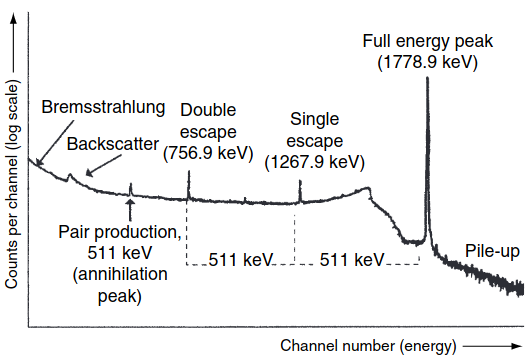
\includegraphics[width = 0.6\textwidth]{Spektrum.png}
\caption{Das Energiespektrum am Beispiel von $^{28}\symup{Al}$. Kurz vor dem Photopeak ist deutlich die Compton-Kante zu erkennen. Die Double und Single escape Peaks können der Paarerzeugung zugeordnet werden \cite{quelle02}.}
\label{fig:tfig8}
\end{figure}
\FloatBarrier
Das Energiespektrum eines monochromatischen Gammastrahlers weist einige Charakteristika auf, welche in Abbildung \ref{fig:tfig8} dargestellt sind.
Wesentliche Bestandteile sind das Compton-Kontinuum, der Rückstreupeak und der Photopeak.
Der Photopeak wird auch Vollenergiepeak genannt, da er durch den Photoeffekt entsteht, bei welchem die Photonen ihre gesamte Energie im Detektor deponieren.
Das Maximum des Photopeaks entspricht also der Energie der Gammastrahlung.

Das Compton-Kontinuum und die Compton-Kante entstehen durch die Compton-Streuung.
Die Compton-Kante entspricht dabei der Energie, welche bei bei einem Winkel von $180°$ übertragen wird, also dem maximalen Energieübertrag, welcher beim Compton-Effekt auftreten kann.
Da das Photon durch die Compton-Streuung nicht annihiliert wird kommt es auch zu Mehrfachstreuungen, sodass die deponierte Energie teilweise auch größer als die der Compton-Kante sein kann.
Aus diesem Grund ist die Compton-Kante keine scharfe Kante, sondern ist leicht verschmiert.

Bei einige Gamma-Quanten kommt es auch zu Wechselwirkungen mit der Abschirmung des Detektors und somit zu Energieverlust.
Diese können von der Abschirmung zurückgestreut werden, sodass sie den Detektor mit geringerer Energie erreichen.
Der dadurch erzeugte Peak wird Rückstreupeak genannt und entspricht einer Energie von
\begin{equation}
    \label{eq:ruckstreu}
E_\text{Rück}= \frac{E_{\gamma}}{1+2\varepsilon}\, .
\end{equation}

Die Double und Single escape Peaks entstehen durch die Paarerzeugung.
Eine Erläuterung zu diesem Prozess ist in Abschnitt \ref{sec:paar} zu finden. 

\section{Durchführung}
Zu Beginn der Messung wird eine kalibrierte $^{152}\symup{Eu}$-Probe vermessen, sodass diese zur Energiekalibrierung genutzt werden kann.
Anschließend wird das Spektrum eines $^{137}\symup{Cs}$-Strahlers aufgenommen, sowie das einer $^{133}\text{Ba}$-Quelle.
Zuletzt wird das Spektrum eines unbekannten Strahlers vermessen, wobei als Probe Bananenchips verwendet werden.

\section{Auswertung}
Im Folgenden werden diese Messwerte ausgewertet. Zuerst wird anhand eines $^{152}\text{Eu}$-Strahlers eine Energiekalibrierung
des verwendeten Germanium-Detektors durchgeführt und die Vollenergienachweiswahrscheinlichkeit bestimmt.
Anschließend wird das Gamma-Spektrum eines $^{137}\text{Cs}$-Strahlers untersucht. Dazu wird dessen Energie bestimmt und die 
Vollenergielinie sowie das Compton-Kontinuum analysiert. 
Weiterhin wird die Aktivität eine $^{133}\text{Ba}$-Strahlers berechnet, wozu die Linieninhalte der einzelnen Spektrallinien 
des Gamma-Spektrums bestimmt werden. 
Abschließend wird das Spektrum des unbekannten Strahlers hinsichtlich der Position und des Inhalts der Spektrallinien untersucht
und die aktiven Isotope des unbekannten Strahlers bestimmt.
\subsection{Energiekalibrierung und Bestimmung der Nachweiswahrscheinlichkeit}
\label{sec:nachweis}
Die Kalibrierung erfolgt anhand eines $^{152}\text{Eu}$-Strahlers.  
Die Aktivität dieses Strahlers betrug am 01.10.2000 $(4130 \pm 60) \, \text{Bq}$. Gemäß des Geseztes des
radioaktiven Zerfalls ist die Aktivität des Strahlers mit der Zerfallskonstante 
$\lambda = 1.623 \cdot 10^{-9} \, \frac{1}{\text{s}}$ \cite{Periodensystem}
am Messtag, dem 26.02.2014
\begin{equation*}
    A(t) = (2079 \pm 30) \, \text{Bq} \, .
\end{equation*}
Der Fehler berechnet sich in dieser und in allem folgenden Berechnungen mit dem 
\texttt{python}-Paket \texttt{uncertainties} \cite{uncertainties}. Alle Abbildungen werden mit dem Paket \texttt{matplotlib}
\cite{Hunter:2007} erstellt.

Das gemessene Spektrum von $^{152}\text{Eu}$ ist in Abbildung \ref{fig:europium-spektrum} dargestellt.
Da in höheren Kanalnummern kein signifikanter Verlauf erkennbar ist, werden nur die ersten 4000 Kanalnummern
dargestellt.
Insgesamt gibt es 8191 Kanäle. Die Messzeit beträgt $4612 \, \text{s}$.
Für die Energiekalibrierung wird die Lage der Peaks bestimmt, wozu die Funktion \texttt{find\_peaks}
des \texttt{Python}-Pakets \texttt{SciPy} \cite{Scipy} verwendet wird. 
Die verwendeten Peaks sind durch die Markierungspunkte in Abbildung \ref{fig:europium-spektrum} dargestellt.
\FloatBarrier
\begin{figure}
\centering
\includegraphics[width = 0.8\textwidth]{europium.pdf}
\caption{Das Spektrum von $^{152}\text{Eu}$. Dargestellt ist die Anzahl der gemessenen Counts in Abhängigkeit von der Kanalnummer.
        Die bestimmten Peaks sind durch die Markierungspunkte dargestellt.
        Aus Gründen der Übersichtlichkeit werden nur die ersten 4000 Kanalnummern verwendet.}
\label{fig:europium-spektrum}
\end{figure}
\FloatBarrier
Für die Energiekalibrierung wird nun jeder Peak in einer Umgebung von 70 Kanalnummern 
an eine Gaußkurve der Form
\begin{equation}
    \label{eq:gaussfit}
    f(x) = a \cdot \text{exp}\left(-\frac{\left(x - \mu\right)^2}{2\sigma^2}\right) + d
\end{equation}
angepasst.
Die entsprechenden Parameter sind in Tabelle \ref{tab:gauss-parameter-europium} angegeben.
\begin{table}[h]
    \centering
    \caption{Parameter des Fits der einzelnen Peaks an eine Gaußkurve zur Energiekalibrierung.}
    \label{tab:gauss-parameter-europium}
    \begin{tabular}{S[table-format=4.2] @{${}\pm{}$} S[table-format=2.2] S[table-format=4.2] @{${}\pm{}$} S[table-format=1.2] S[table-format=1.3] @{${}\pm{}$} S[table-format=1.3] S[table-format=3.2] @{${}\pm{}$} S[table-format=1.2]}
        \toprule
        \multicolumn{2}{c}{$a$} & \multicolumn{2}{c}{$\mu$} & \multicolumn{2}{c}{$\sigma$} & \multicolumn{2}{c}{$d$} \\
        \midrule
        7532.93 & 29.43 &  252.61  & 0.01  &  0.986 & 0.005  &  152.56 & 3.92 \\
        1215.66 & 11.58 &  501.84  & 0.01  &  1.045 & 0.012  &  69.25  & 1.60 \\
        2741.51 & 6.22  &  703.66  & 0.01  &  1.115 & 0.003  &  37.34  & 0.89 \\
        85.85   & 5.90  &  751.14  & 0.08  &  1.037 & 0.083  &  31.57  & 0.81 \\
        177.47  & 5.11  &  839.09  & 0.03  &  1.041 & 0.035  &  30.37  & 0.70 \\
        235.79  & 4.75  &  905.70  & 0.03  &  1.192 & 0.028  &  27.375 & 0.70 \\
        456.98  & 4.04  &  1584.78 & 0.01  &  1.334 & 0.014  &  20.87  & 0.64 \\
        137.52  & 3.92  &  1764.13 & 0.04  &  1.337 & 0.045  &  19.87  & 0.62 \\
        402.70  & 3.70  &  1960.21 & 0.02  &  1.498 & 0.016  &  10.72  & 0.62 \\
        238.49  & 6.90  &  2207.39 & 0.05  &  1.376 & 0.047  &  11.38  & 1.10 \\
        316.73  & 2.74  &  2260.57 & 0.02  &  1.518 & 0.015  &  9.17   & 0.46 \\
        367.98  & 2.47  &  2860.91 & 0.01  &  1.611 & 0.013  &  1.19   & 0.43 \\
        \bottomrule
    \end{tabular}
\end{table}
\noindent
Die Kanalnummer der einzelnen Peaks ist jeweils durch den Parameter $\mu$ gegeben.
Durch einen Vergleich dieser Parameter mit den Werten der Datenbank \cite{Datenbank}
kann den Emissionslinien die jeweilige Gammaenergie und Emissionswahrscheinlichkeit zugeordnet werden.
Die Zuordnung ist in Tabelle \ref{tab:europium-datenbank} angegeben.
\begin{table}[h]
    \centering
    \caption{Zuordnung der Emissionslinien zu der jeweiligen Gammaenergie und Emissionswahrscheinlichkeit
        durch Vergleich mit den Werten der Datenbank \cite{Datenbank}.}
    \label{tab:europium-datenbank}
    \begin{tabular}{S[table-format=4.2] @{${}\pm{}$} S[table-format=1.2] c c}
        \toprule
        \multicolumn{2}{c}{$\mu$} & {$E_{\gamma} / \text{keV}$} & {$\text{P} / \%$} \\
        \midrule
        252.61  & 0.01  & 121.7812 & 28.41 \\
        501.84  & 0.01  & 244.6974 & 7.55  \\ 
        703.66  & 0.01  & 344.2785 & 26.59 \\  
        751.14  & 0.08  & 367.7891 & 0.862 \\  
        839.09  & 0.03  & 411.1165 & 2.238 \\  
        905.70  & 0.03  & 443.965  & 3.120 \\ 
        1584.78 & 0.01  & 778.9045 & 12.97 \\  
        1764.13 & 0.04  & 867.380  & 4.243 \\ 
        1960.21 & 0.02  & 964.079  & 14.50 \\ 
        2207.39 & 0.05  & 1085.837 & 10.13 \\  
        2260.57 & 0.02  & 1112.076 & 13.41 \\  
        2860.91 & 0.01  & 1408.013 & 20.85 \\  
        \bottomrule
    \end{tabular}
\end{table}
\noindent
Anhand der Wertepaare aus Kanalnummer und Gammaenergie wird nun eine lineare Ausgleichsrechnung
durchgeführt, welche in Abbildung \ref{fig:ausgleichsrechnung-europium} dargestellt ist.
\FloatBarrier
\begin{figure}
    \centering
    \includegraphics[width = 0.8\textwidth]{LineareRegression.pdf}
    \caption{Ausgleichsrechnung zur Energiekalibrierung mit den Wertepaaren aus Kanalnummer und Gammaenergie.}
    \label{fig:ausgleichsrechnung-europium}
\end{figure}
\FloatBarrier
Die Parameter dieser Ausgleichsrechnung ergeben sich zu
\begin{align}
    a &= (0.493  \pm 0.000) \, \text{keV} \, , \\
    b &= (-2.846 \pm 0.100) \, \text{keV} \, .
\end{align}
Die Energiekalibrierung kann daher mit der Kanalnummer $x$ über 
\begin{equation}
    \label{eq:kalibrierung}
    E_\gamma (x) = a \cdot x + b 
\end{equation}
erfolgen.

Zur Bestimmung der Vollenergienachweiswahrscheinlichkeit muss zuerst der Inhalt $I$
der Peaks berechnet werden. Dazu wird die Gaußfunktion \eqref{eq:gaussfit} integriert
\begin{equation}
    \label{eq:inhalt}
    I = \int_{-\infty}^{\infty} a \cdot \text{exp}\left(-\frac{\left(x - \mu\right)^2}{2\sigma^2}\right) = \sqrt{2 \pi} \cdot a \cdot \sigma
\end{equation}
wobei die Konstante $d$ vorher abgezogen wird. 
Die so berechneten Linieninhalte sind mit der entsprechenden Gammaenergie und den verwendeten Parametern in 
Tabelle \ref{tab:europium-inhalt} angegeben.
\begin{table}[h]
    \centering
    \caption{Linieninhalte der einzelnen Peaks mit den entsprechenden Parametern die bei der Berechnung verwendet werden sowie die zugehörige Gammaenergie.}
    \label{tab:europium-inhalt}
    \begin{tabular}{l S[table-format=4.2] @{${}\pm{}$} S[table-format=2.2] S[table-format=1.3] @{${}\pm{}$} S[table-format=1.3] S[table-format=5.3] @{${}\pm{}$} S[table-format=3.3]}
        \toprule
        {$E_{\gamma} / \text{keV}$} & \multicolumn{2}{c}{$\mu$} & \multicolumn{2}{c}{$\sigma$} & \multicolumn{2}{c}{$I$}  \\
        \midrule
        121.7812 & 7532.93 & 29.43 &  0.986 & 0.005  &  18619.025 & 111.976 \\
        244.6974 & 1215.66 & 11.58 &  1.045 & 0.012  &  3184.586  & 46.554  \\
        344.2785 & 2741.51 & 6.22  &  1.115 & 0.003  &  7663.254  & 26.703  \\
        367.7891 & 85.85   & 5.90  &  1.037 & 0.083  &  223.256   & 23.550  \\
        411.1165 & 177.47  & 5.11  &  1.041 & 0.035  &  463.017   & 20.431  \\
        443.965  & 235.79  & 4.75  &  1.192 & 0.028  &  704.774   & 21.805  \\
        778.9045 & 456.98  & 4.04  &  1.334 & 0.014  &  1528.046  & 20.790  \\
        867.380  & 137.52  & 3.92  &  1.337 & 0.045  &  460.976   & 20.199  \\
        964.079  & 402.70  & 3.70  &  1.498 & 0.016  &  1511.606  & 21.330  \\
        1085.837 & 238.49  & 6.90  &  1.376 & 0.047  &  822.613   & 36.596  \\
        1112.076 & 316.73  & 2.74  &  1.518 & 0.015  &  1204.928  & 16.049  \\
        1408.013 & 367.98  & 2.47  &  1.611 & 0.013  &  1485.888  & 15.338  \\
        \bottomrule 
    \end{tabular}
\end{table}
\noindent
Die Vollenergienachweiswahrscheinlichkeit $Q$ wird nun bestimmt, indem die Theoriewerte des Peakinhalts berechnet werden
und der Quotient aus experimentellem und theoretischem Wert gebildet wird
\begin{equation}
    Q = \frac{I}{I_\text{Theorie}} \, .
\end{equation}
Der theoretische Wert berechnet sich mit der Emissionswahrscheinlichkeit $P$, der Aktivität $A$, dem Raumwinkelanteil $\Omega / 4 \pi$ und der Messzeit $t$ durch
\begin{equation}
    \label{eq:inhalt_theorie}
    I_\text{Theorie} = P \cdot \frac{\Omega}{4 \pi} \cdot A \cdot t \, .
\end{equation}
Zunächst muss daher der Raumwinkelanteil bestimmt werden. 
Dieser berechnet sich gemäß Gleichung \eqref{eq:raumwinkel}. 
Der Abstand zum Detektor betrug $a = 8 \, \text{cm}$. Wird der Abstand von $1,5 \, \text{cm}$ zwischen Aluminium-Haube und Detektor
und der Radius $r = 2,25 \, \text{cm}$ des Detektorvolumens berücksichtigt, so ergibt sich
der Raumwinkelanteil zu 
\begin{equation}
    \frac{\Omega}{4 \pi} \approx 0.013459 \, .
\end{equation}
Die berechneten Theoriewerte und die berechnete Nachweiswahrscheinlichkeit sind zusammen mit den entsprechenden Gammaenergien
und experimentellem Werten in Tabelle \ref{tab:nachweis-europium} angegeben.
\begin{table}[h]
    \centering
    \caption{Theoretisch berechnete und experimentell bestimmte Linieninhalte der einzelnen Peaks sowie der Quotient $Q$ dieser Werte als Maß für die Nachweiswahrscheinlichkeit. 
            Angegeben sind außerdem die Gammaenergien.}
    \label{tab:nachweis-europium}
    \begin{tabular}{l S[table-format=5.3] @{${}\pm{}$} S[table-format=3.3] S[table-format=5.3] @{${}\pm{}$} S[table-format=3.3] S[table-format=1.3] @{${}\pm{}$} S[table-format=1.3]}
        \toprule
        {$E_{\gamma} / \text{keV}$}  & \multicolumn{2}{c}{$I$} & \multicolumn{2}{c}{$I_\text{Theorie}$} & \multicolumn{2}{c}{$Q$}  \\
        \midrule
        121.7812 & 18619.025 & 111.976 &  36659.379 & 532.582  &  0.508 & 0.008 \\
        244.6974 & 3184.586  & 46.554  &  9742.285  & 141.534  &  0.327 & 0.007 \\
        344.2785 & 7663.254  & 26.703  &  34310.907 & 498.464  &  0.223 & 0.003 \\
        367.7891 & 223.256   & 23.550  &  1112.298  & 16.159   &  0.201 & 0.021 \\
        411.1165 & 463.017   & 20.431  &  2887.845  & 41.954   &  0.160 & 0.007 \\
        443.965  & 704.774   & 21.805  &  4025.951  & 58.488   &  0.175 & 0.006 \\
        778.9045 & 1528.046  & 20.790  &  16736.084 & 243.139  &  0.091 & 0.002 \\
        867.380  & 460.976   & 20.199  &  5475.035  & 79.540   &  0.084 & 0.004 \\
        964.079  & 1511.606  & 21.330  &  18710.348 & 271.821  &  0.081 & 0.002 \\
        1085.837 & 822.613   & 36.596  &  13071.436 & 189.900  &  0.063 & 0.003 \\
        1112.076 & 1204.928  & 16.049  &  17303.846 & 251.388  &  0.070 & 0.001 \\
        1408.013 & 1485.888  & 15.338  &  26904.190 & 390.860  &  0.055 & 0.001 \\
        \bottomrule 
    \end{tabular}
\end{table}
\noindent
In Abbildung \ref{fig:potenzfunktion} ist die Nachweiswahrscheinlichkeit in Abhängigkeit 
von der Gammaenergie dargestellt. An die Messwerte wird nun eine Potenzfunktion der Form
\begin{equation}
    \label{eq:potenz}
    Q (E_\gamma) = a \cdot {E_\gamma}^b
\end{equation}
angepasst. Die Parameter dieser Rechnung ergeben sich zu
\begin{align}
    \label{eq:parameter_potenz}
    a &= 47.5425 \pm 2.2181 \, , \\
    b &= -0.9305 \pm 0.0075 \, .
\end{align}
\FloatBarrier
\begin{figure}
\centering
\includegraphics[width = 0.8\textwidth]{Potenzfunktion.pdf}
\caption{Wertepaare aus Gammaenergie und Nachweiswahrscheinlichkeit und angepasste Potenzfunktion.}
\label{fig:potenzfunktion}
\end{figure}
\FloatBarrier
\subsection{Untersuchung des monochromatischen Gammaspektrums von \texorpdfstring{$^{137}\text{Cs}$}{Cs}}
Die Messwerte von $^{137}\text{Cs}$ wird zunächst anhand von Gleichung \eqref{eq:kalibrierung}
kalibriert. Das resultierende Energiespektrum ist in Abbildung \ref{fig:energie-caesium} dargestellt.
Verwendet werden nur die Energien bis $1000 \, \text{keV}$, da die Ergebnisse bei höheren Energien nicht mehr
signifikant sind. Die Messzeit betrug $3103 \, \text{s}$.
\FloatBarrier
\begin{figure}
\centering
\includegraphics[width = 0.8\textwidth]{caesium.pdf}
\caption{Das Energiespektrum von $^{137}\text{Cs}$. 
        Aus Gründen der Übersichtlichkeit werden nur Energien bis $1000 \, \text{keV}$ dargestellt.}
\label{fig:energie-caesium}
\end{figure}
\FloatBarrier
Die Vollenergielinie befindet sich bei Kanalnummer 1347. Zur Bestimmung des Inhalts 
wird sie an eine Gaußkurve \eqref{eq:gaussfit} angepasst, wobei sich die Parameter
\begin{align}
    a &= (4106.160 ± 10.298) \, \\
    \mu &= (661.349 ± 0.002) \, \text{keV} \\
    \sigma &= (0.600 ± 0.002) \, \text{keV} \\
    d &= (4.479 ± 3.163) \,
\end{align}
ergeben.
Die experimentell bestimmte Energie ist durch $\mu$ gegeben
\begin{equation}
    E_\gamma = (661.349 ± 0.002) \, \text{keV} \, .
\end{equation}
Der theoretische Wert, welcher der Datenbank \cite{Datenbank} entnommen wird, ist $661.657 \, \text{keV}$
mit einer Emissionswahrscheinlichkeit von $P = 84.99 \, \%$.
Die Halbwertsbreite und Zehntelwertsbreite der Gaußkurve kann aus Abbildung \ref{fig:caesium-gauss}
abgelesen werden
\begin{align*}
    E_{1/2}  &= (1.48 \pm 0.28) \, \text{keV} \, , \\
    E_{1/10} &= (2.71 \pm 0.28) \, \text{keV} \, ,
\end{align*}
wobei eine Ablesefehler von $0.2 \, \text{keV}$ angenommen wird.
\begin{figure}
\centering
\includegraphics[width = 0.8\textwidth]{caesium_gauss.pdf}
\caption{Messwerte des Energiespektrums von $^{137}\text{Cs}$ im Bereich der Vollenergielinie sowie angepasste Gaussfunktion.
    Die Halbwertsbreite kann über die grüne Linie, die Zehntelwertsbreite über die rote Linie abgelesen werden.}
\label{fig:caesium-gauss}
\end{figure}
Das Verhältnis dieser Werte beträgt
\begin{equation}
    \frac{E_{1/2}}{E_{1/10}} = 0.55 \pm 0.12 \, .
\end{equation}
Die Halb- und Zehntelwertsbreite kann jedoch aus auch den Parametern der Gausskurve über 
\begin{align}
    E_{1/2}  &= 2 \sqrt{2 \ln (2)} \cdot \sigma \, , \\
    E_{1/10} &= 2 \sqrt{2 \ln (10)} \cdot \sigma \, ,
\end{align}
berechnet werden. Das Verhältnis dieser Werte ist unabhängig vom Parameter $\sigma$
und beträgt
\begin{equation}
    \left(\frac{E_{1/2}}{E_{1/10}}\right)_\text{Theorie} \approx 0.5486 \, .
\end{equation}
Der Inhalt der Vollenergielinie (VEL) ergibt sich mit Gleichung \eqref{eq:inhalt} zu
\begin{equation}
    I_\text{VEL} = 6176 \pm 24 \, .
\end{equation}
Die Lage der Compton-Kante wird wieder über die \texttt{SciPy}-Funktion \texttt{find\_peaks} bestimmt. 
Sie befindet sich bei Kanalnummer 965 mit einer Energie von $472.5 \, \text{keV}$.
Der theoretische Wert der Compton-Kante wird mit Gleichung \eqref{eq:compton} zu
\begin{equation}
    E_{\gamma_\text{Compton}} = 477.334 \, \text{keV} 
\end{equation}
bestimmt.
Die Energie des Rückstreupeaks wird analog bestimmt und ergibt sich zu $186 \, \text{keV}$.
Der theoretische Wert berechnet sich mit Formel \eqref{eq:ruckstreu}
\begin{equation}
    E_{\gamma_\text{Rückstreu}} = 184.323 \, \text{keV} \, .
\end{equation}
Anschließend wird der Inhalt des Compton-Kontinuums bestimmt.
Dazu werden die Messwerte von Kanalnummer 925 bis 950 knapp unterhalb der Compton-Kante 
an den Wirkungsquerschnitt \eqref{eq:diffwirkung} angepasst wodurch sich der konstante Faktor
\begin{equation}
    \kappa = 10.577 ± 0.161
\end{equation}
ergibt. Mit diesem Faktor kann der Wirkungsquerschnitt nun im Energiebereich des Compton-Kontinuums
von $51\, \text{keV}$ bis $965 \, \text{keV}$ 
numerisch integriert werden, wozu die \texttt{SciPy}-Funktion \texttt{integrate.quad} verwendet wird.
Der Inhalt des Compton-Kontinuums (CK) berechnet sich zu 
\begin{equation}
    I_\text{CK}  = 43592.368 \, .
\end{equation}
Aus dem Verhältnis der Absorptionswahrscheinlichkeiten von Compton- und Photopeak 
kann ein theoretischer Vergleichswert für das Verhältnis von $I_\text{VEL}$ und $I_\text{CK}$
bestimmt werden, sodass eine Überprüfung der experimentellen Ergebnisse möglich ist. 
Die Absorptionswahrscheinlichkeit berechnet sich mit dem Extinktionskoeffizienten $\mu$ und der Länge des 
Detektors $l$ über 
\begin{equation}
    p = 1 - \text{e}^{- \mu l} \, .
\end{equation}
Die Extinktionskoeffizienten können über die Energie von Compton-Kante und Photopeak aus entsprechenden Grafiken abgelesen werden und haben 
die Werte 
\begin{align*}
    \mu_\text{Compton}  &= 0.41 \frac{1}{\text{cm}} \, ,\\
    \mu_\text{Photo}  &= 0.008 \frac{1}{\text{cm}} \, ,
\end{align*}
sodass sich für die Absorptionswahrscheinlichkeiten
\begin{align*}
    p_\text{Compton}  &= 0.79790 \, ,\\
    p_\text{Photo}  &= 0.03072 \, .
\end{align*}
ergibt.
Das Verhältnis der theoretischen und experimentell bestimmten Werte ist daher 
\begin{equation}
    \left(\frac{I_\text{VEL}}{I_\text{CK}}\right)_\text{Theorie} = \frac{p_\text{Photo}}{p_\text{Compton}} = 0.03850 \qquad \qquad \left(\frac{I_\text{VEL}}{I_\text{CK}}\right)_\text{Experiment} = 0.1417 \, . 
\end{equation}

\subsection{Aktivitätsbestimmung einer \texorpdfstring{$^{133}\text{Ba}$}{Cs}--Probe}
Wie schon bei $^{137}\text{Cs}$ wird das Spektrum der $^{133}\text{Ba}$ zunächst anhand von
Gleichung \eqref{eq:kalibrierung} kalibriert. Das Energiespektrum bis $600 \, \text{keV}$ ist in Abbildung \ref{fig:energie-barium}
dargestellt. Die Peaks werden ebenfalls mit \texttt{scipy.find\_peaks} bestimmt und sind durch die Punkte markiert.
%\FloatBarrier
\begin{figure}
\centering
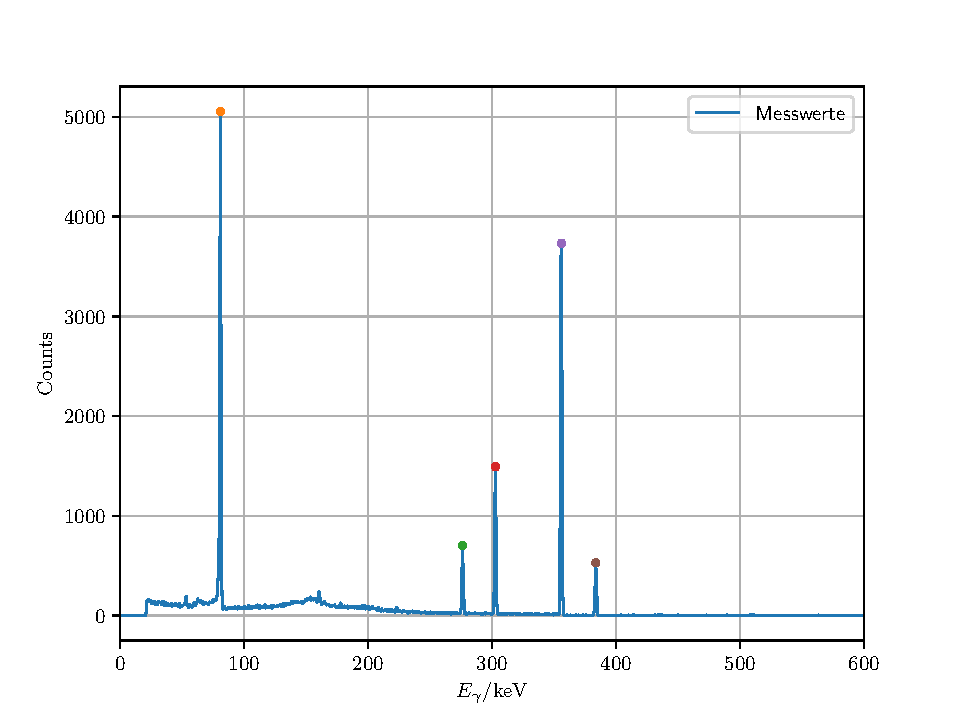
\includegraphics[width = 0.8\textwidth]{barium.pdf}
\caption{Das Energiespektrum von $^{133}\text{Ba}$. 
        Aus Gründen der Übersichtlichkeit werden nur Energien bis $600 \, \text{keV}$ dargestellt.}
\label{fig:energie-barium}
\end{figure}
%\FloatBarrier
Die Messzeit betrug bei dieser Probe 3534 s. In Analogie zur Auswertung des Europium-Spektrums 
wird nun jeweils eine Gaussfunktion \eqref{eq:gaussfit} an die Messwerte in einer Umgebung von 70 Kanalnummern des Peaks angepasst.
Die so gewonnenen Parametern werden mit der Datenbank \cite{Datenbank} abgeglichen. Die Gammaenergien und Emissionswahrscheinlichkeiten
sind zusammen mit dem Parameter $\mu$ in Tabelle \ref{tab:barium-datenbank} angegeben.
\begin{table}[h]
    \centering
    \caption{Zuordnung der Emissionslinien zu der jeweiligen Gammaenergie und Emissionswahrscheinlichkeit
        durch Vergleich mit den Werten der Datenbank \cite{Datenbank}.}
    \label{tab:barium-datenbank}
    \begin{tabular}{S[table-format=3.3] @{${}\pm{}$} S[table-format=1.3] S[table-format=3.4] S[table-format=2.2]}
        \toprule
        \multicolumn{2}{c}{$\mu / \text{keV}$} & {$E_{\gamma} / \text{keV}$} & {$\text{P} / \%$} \\
        \midrule
        80.933  & 0.008 & 80.9979  & 33.31 \\
        276.250 & 0.005 & 276.3989 & 7.13  \\
        302.710 & 0.002 & 302.8508 & 18.31 \\
        355.848 & 0.002 & 356.0129 & 62.05 \\
        383.640 & 0.002 & 383.8458 & 8.94  \\
        \bottomrule
    \end{tabular}
\end{table}
\noindent
Zwischen dem Inhalt der Peaks und der Aktivität besteht gemäß Gleichung \ref{eq:inhalt_theorie}
ein linearer Zusammenhang. Der Proportionalitätsfaktor ist
\begin{equation}
    \rho = P \cdot \frac{\Omega}{4 \pi} \cdot t \cdot Q \, .
\end{equation}
Der Raumwinkelanteil und der relevante Zusammenhang zur Bestimmung der Nachweiswahrscheinlichkeit $Q$ ist bereits aus Abschnitt \ref{sec:nachweis} bekannt \eqref{eq:potenz},
wobei die dort bestimmten Parameter \eqref{eq:parameter_potenz} verwendet werden. 

Es wird daher eine lineare Ausgleichsrechnung durchgeführt, welche in Abbildung \ref{fig:ausgleichsrechnung-barium} dargestellt ist.
Über den Parameter $a$ erhält man so die Aktivität.
%\FloatBarrier
\begin{figure}
    \centering
    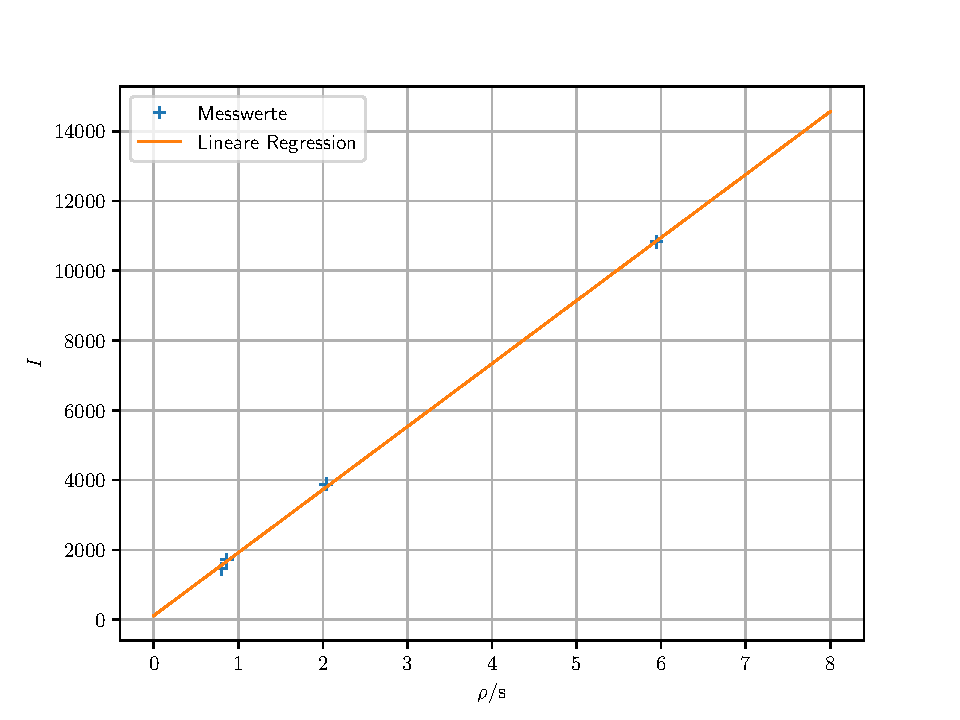
\includegraphics[width = 0.8\textwidth]{LineareRegression_Barium.pdf}
    \caption{Ausgleichsrechnung zur Bestimmung der Aktivität von $^{133}\text{Ba}$ mit den Wertepaaren aus Proportionalitätsfaktor und Inhalt der Peaks $I$.}
    \label{fig:ausgleichsrechnung-barium}
\end{figure}
%\FloatBarrier
Die verwendeten Wertepaare sind in Tabelle \ref{tab:barium-inhalt} angegeben. Für die Ausgleichsrechnung
wird der Wert bei $80.9970 \, \text{keV}$ nicht berücksichtigt, da die Nachweiswahrscheinlichkeit wird bei dieser Energie zu ungenau wird.
Die Parameter dieser Ausgleichsrechnung ergeben sich zu
\begin{align}
    a &= (1805.949 \pm 24.054) \, \text{Bq} \, , \\
    b &= (115.360 \pm 76.887) \, .
\end{align}
\FloatBarrier
\begin{table}[h]
    \centering
    \caption{Linieninhalte der einzelnen Peaks mit den entsprechenden Parametern die bei der Ausgleichsrechnung verwendet werden sowie die zugehörige Gammaenergie, Emissionswahrscheinlichkeit und Nachweiswahrscheinlichkeit}
    \label{tab:barium-inhalt}
    \begin{tabular}{S[table-format=3.4] S[table-format=2.2] S[table-format=5.3] @{${}\pm{}$} S[table-format=2.3] S[table-format=1.4] @{${}\pm{}$} S[table-format=1.5]}
        \toprule
        {$E_{\gamma} / \text{keV}$} & {$P / \%$} & \multicolumn{2}{c}{$I$} & \multicolumn{2}{c}{$Q$}  \\
        \midrule
        276.3989 & 7.13  & 1714.485  & 24.480 &  0.2544 & 0.0160 \\
        302.8508 & 18.31 & 3886.379  & 18.086 &  0.2335 & 0.0148 \\
        356.0129 & 62.05 & 10827.332 & 42.798 &  0.2009 & 0.0129 \\
        383.8458 & 8.94  & 1454.508  & 6.904  &  0.1874 & 0.0121 \\
        \bottomrule 
    \end{tabular}
\end{table}
\FloatBarrier
\noindent
\subsection{Nuklididentifikation und Aktivitätsbestimmung eines unbekannten Strahlers}
Als Anwendung des Germanium-Detektors werden nun Bananenchips als Probe untersucht.

Bei der Messung des Spektrums wurde jedoch nicht nur das Spektrum dieses unbekannten Strahlers, sondern auch ein Untergrundspektrum gemessen.
Das Untergrundspektrum wurde zusätzlich in einer Messung ohne Probe aufgenommen und muss zuerst
abgezogen werden. 

Relevant für die Analyse eines Spektrums sind jedoch nur die Peaks. Daher werden zuerst 
die Kanalnummer der Peaks des Untergrundspektrums bestimmt. Die Anzahl der Counts an dieser Kanalnummer und in einer 
Umgebung von 20 Kanalnummern wird dann vom Spektrum der Probe abgezogen.
Außerdem werden die ersten 1000 Kanäle nicht berücksichtigt, da dort ein starkes Untergrundrauschen besteht, wodurch 
keine genaue Analyse möglich ist.

Zu Bestimmung der Kanalnummern der Peaks des Untergrundspektrums wird wieder die Funktion \texttt{SciPy.find\_peaks} verwendet.
Nachdem der Untergrund vom Spektrum der Probe abgezogen ist, wird erneut eine Energiekalibrierung durchgeführt. 
Das Energiespektrum der Probe ist in Abbildung \ref{fig:banane_energie} dargestellt, die gefundenen Peaks sind durch einen Punkt markiert.
%\FloatBarrier
\begin{figure}
    \centering
    \includegraphics[width = 0.8\textwidth]{banane_energie.pdf}
    \caption{Das Energiespektrum des unbekannten Strahlers.}
\label{fig:banane_energie}
\end{figure}
%\FloatBarrier 

Die Peaks werden nun mit einer Gausskurve \eqref{eq:gaussfit} gefittet, um den Inhalt der Linien zu bestimmen.
Die relevanten Größen sowie der Inhalt der Linien sind in Tabelle \ref{tab:banane-inhalt} angegeben.
\begin{table}[h]
    \centering
    \caption{Linieninhalte der einzelnen Peaks mit den entsprechenden Parametern sowie die zugehörige Gammaenergie.}
    \label{tab:banane-inhalt}
    \begin{tabular}{S[table-format=4.3] @{${}\pm{}$} S[table-format=1.3] S[table-format=4.3] @{${}\pm{}$} S[table-format=2.3]}
        \toprule
        \multicolumn{2}{c}{$E_{\gamma} / \text{keV}$} & \multicolumn{2}{c}{$I$}  \\
        \midrule
         583.070 & 0.071 & 76.993   & 23.907 \\
        1377.417 & 0.106 & 61.208   & 12.557 \\
        1408.044 & 0.076 & 28.024   & 7.310 \\
        1460.589 & 0.014 & 1119.267 & 36.461 \\
        1729.828 & 0.057 & 34.876   & 8.015 \\
        1764.255 & 0.037 & 195.539  & 18.586 \\
        \bottomrule 
    \end{tabular}
\end{table}
\noindent
Im gemessenen Energiespektrum besonders auffällig ist die Linie bei $160.589 \, \text{keV}$, die 
auch den größten Linieninhalt hat. Das Spektrum des Strahlers mit dieser Spektrallinie ist daher das Dominierende.
Durch Abgleich der Energie mit der Datenbank \cite{Datenbank} kann diese Linie dem 
Spektrum von $^{40}\text{K}$ zugeordnet werden, welches bei einer Energie $E_\gamma = 1640.882 \, \text{keV}$ eine Spektrallinie
mit einer Emissionswahrscheinlichkeit von $10.5 \%$ hat.

\section{Diskussion}
Zur Untersuchung des Germaniumdetektors wurde zunächst mit einem $^{152}\text{Eu}$-Strahler eine Energiekalibrierung 
durchgeführt und die Vollenergienachweiswahrscheinlichkeit bestimmt. Dann wurde das Gamma-Spektrum eines $^{137}\text{Cs}$-Strahlers analysiert
und aus dem Gamma-Spektrum von $^{133}\text{Ba}$ dessen Aktivität bestimmt. 
Abschließend wurde das Gamma-Spektrum von Bananenchips untersucht. \\

Die Unsicherheit der Parameter der linearen Ausgleichsrechnung zur Energiekalibrierung ist nur sehr klein, 
was auf eine hohe Auflösung des Detektors schließen lässt. Auch die Unsicherheiten bei der Bestimmung der Vollenergienachweiswahrscheinlichkeit 
sind nur gering. Die verwendete Potenzfunktion beschreibt die Energieabhängigkeit daher gut.

Die Abweichung der experimentell bestimmten Energie der Linie des $^{137}\text{Cs}$-Spektrums
vom Theoriewert der Datenbank \cite{Datenbank} beträgt nur $\num{0.0465}$ \%, was auf die hohe Auflösung des Detektors 
zurückzuführen ist. 
Auch die Beschreibung des Peaks durch eine Gausskurve ist sehr genau. Dies wird ersichtlich, wenn das 
experimentell bestimmte Verhältnis von Halb- und Zehntelwertsbreite mit dem theoretischen verglichen wird. 
Die Abweichung beider Werte beträgt nur $\num{0.462}$ \%.
Auch die Lage der Compton-Kante und des Rückstreupeaks wurde mit hoher Genauigkeit bestimmt, hier beträgt
die Abweichung vom Literaturwert $\num{1.01}$ \% bzw. $\num{0.91}$ \%.
Das experimentell bestimmte Verhältnis der Inhalte der Vollenergielinie und des Compton-Kontinuums 
weist jedoch eine Abweichung von $\num{267.99}$ \% auf. Der Grund dafür ist, das in der theoretischen Berechnung über den 
Extinktionskoeffizienten nicht berücksichtigt wird, dass beim Compton-Effekt Mehrfachstreuung 
auftritt. Die mehrfach gestreuten Photonen können dann über den Photoeffekt wechselwirken.
Dadurch steigt der Inhalt der Vollenergielinie, während der Inhalt des Compton-Kontinuums sinkt, sodass das 
Verhältnis ein anderes ist als das berechnete.  

Die Aktivitätsbestimmung des $^{133}\text{Ba}$-Strahlers ist aufgrund der hohen Energieauflösung des Detektors mit hoher Signifikanz möglich.
Der Vergleich mit der Literatur \cite{Bundesamt} bestätigt die Annahme, dass es sich bei dem unbekannten Spektrum der Bananenchips 
hauptsächlich um $^{40}\text{K}$ handelt. Bananen enthalten natürlicherweise Kalium, welches zu einem kleinen Anteil 
aus dem radioaktiven Isotop $^{40}\text{K}$ besteht.

\nocite{wingate}
\nocite{*}
\printbibliography
\end{document}
